\documentclass{article}
\usepackage[margin=0.70in]{geometry}
\usepackage[utf8]{inputenc}
\usepackage{hyperref}
\usepackage{graphicx}
\usepackage{enumitem}
\title{CIS581 Project 3: Image Stitching and Seam Removal}
\author{Paritosh Kelkar }
\date{\today}
\begin{document}


\maketitle

\newpage

\section*{Seam Carving}

\begin{figure}[h]
\centering
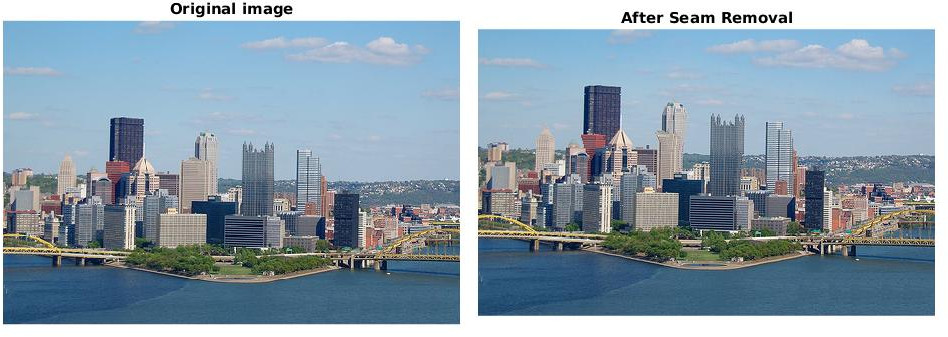
\includegraphics[scale=0.4]{result_afterResize.jpg} 
\label{fig_seamResult}
\caption{The resized image is 50 rows and columns short}
\end{figure}

\begin{figure}[h]
\centering
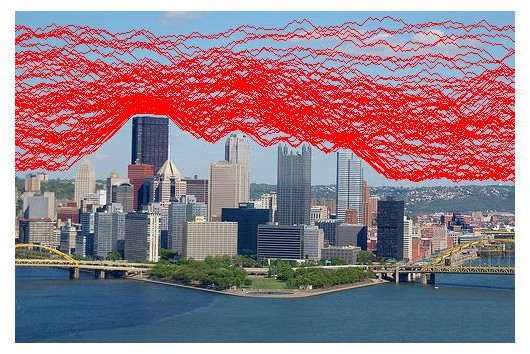
\includegraphics[scale=0.4]{horSeamRemoval.jpg}
\label{fig_seamHorResult}
\caption{The seams that are deleted for deletion of rows}
\end{figure}



\begin{figure}[h]
\centering
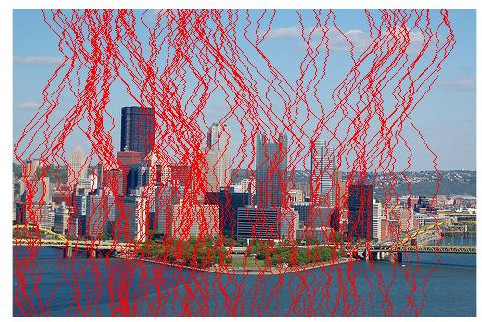
\includegraphics[scale=0.4]{verSeamRemoval.jpg}
\label{fig_seamVerResult}
\caption{The seams that are deleted for deletion of columns}
\end{figure}

\indent It can be clearly seen that this particular image is a good example to show horizontal seam removal. This is because of the relatively low energy features - the cloud and the sky. Seams removed from these regions alter the net Energy of the image the least. While removing vertical seams, it can be seen that the buildings will be affected as there is no way around this. The buildings represent regions of high energy and they extend from the left to the right of the image. Therefore a vertical seam will end up passing through some buildings.

\newpage

\section*{Image Stitching}


\indent These images were taken from a project in CMU doing image stitching. The part of my code that does the actual stitching after the transformations are obtained is taken from matlab's example stitching code.\\
Few parameters that I was tweaking while I did the project:
\begin{itemize}[noitemsep, nolistsep]
\item The number of points to be returned by ANMS
\item The $sigma$ of the Gaussian Kernel used in feat{\_}desc
\item The confidence metric to consider a match as a valid match in feat{\_}match
\item The margin for the considering inliers in ransac{\_}est{\_}homography
\end{itemize}

\subsection*{Future Work}
\indent I wanted to work on making my feature matching more robust by going forward and backward in comparisons to ensure unique matches among descriptors. I also didnt have time to implement geometric invariant descriptors- that would better performance. I also haven't taken into account vertical stitches. These are some areas I could work on to make my stitching more robust. 

\subsection*{Results}
\begin{figure}[h]
\centering
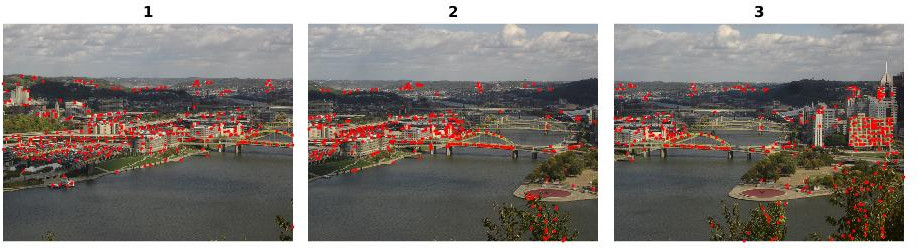
\includegraphics[scale=0.4]{pitt_postANMS.jpg} 
\label{fig_pittPostANMS}
\caption{Corners considered After ANMS for each image}
\end{figure}


\begin{figure}[h]
\centering
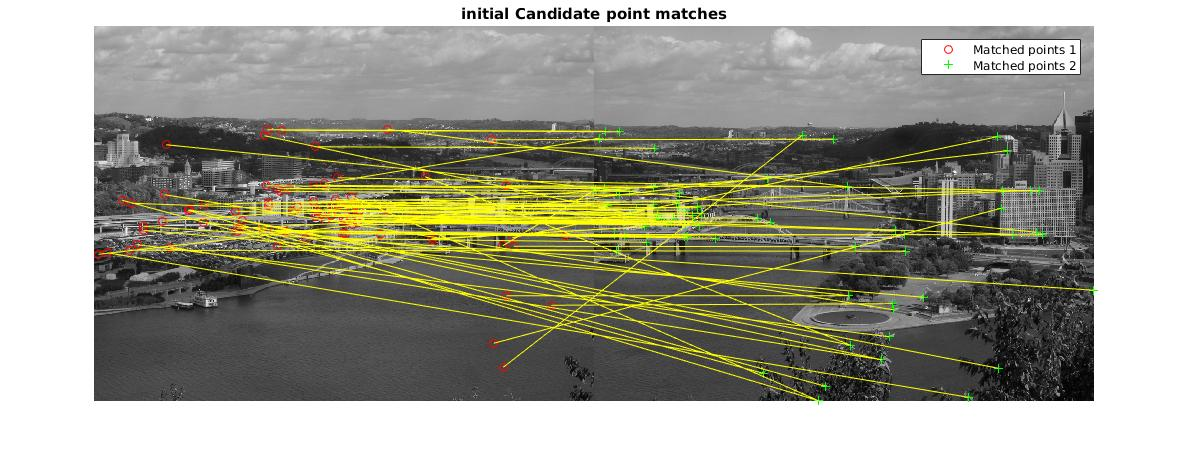
\includegraphics[scale=0.4]{pitt_initialMatches.jpg} 
\label{fig_pittInitMatches}
\caption{Initial matches as provided by the feat{\_}match. Notice the crisscross outliers}
\end{figure}

\begin{figure}[H]
\centering
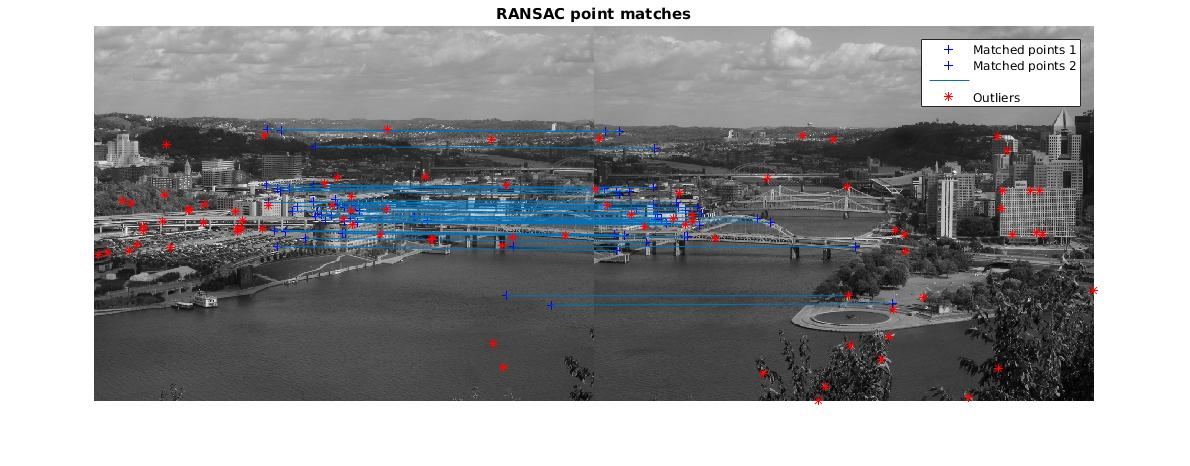
\includegraphics[scale=0.4]{pitt_postRansac.jpg}
\label{fig_pittPostRansac}
\caption{The best points selected after RANSAC. Notice the outliers that have been rejected}
\end{figure}



\begin{figure}[H]
\centering
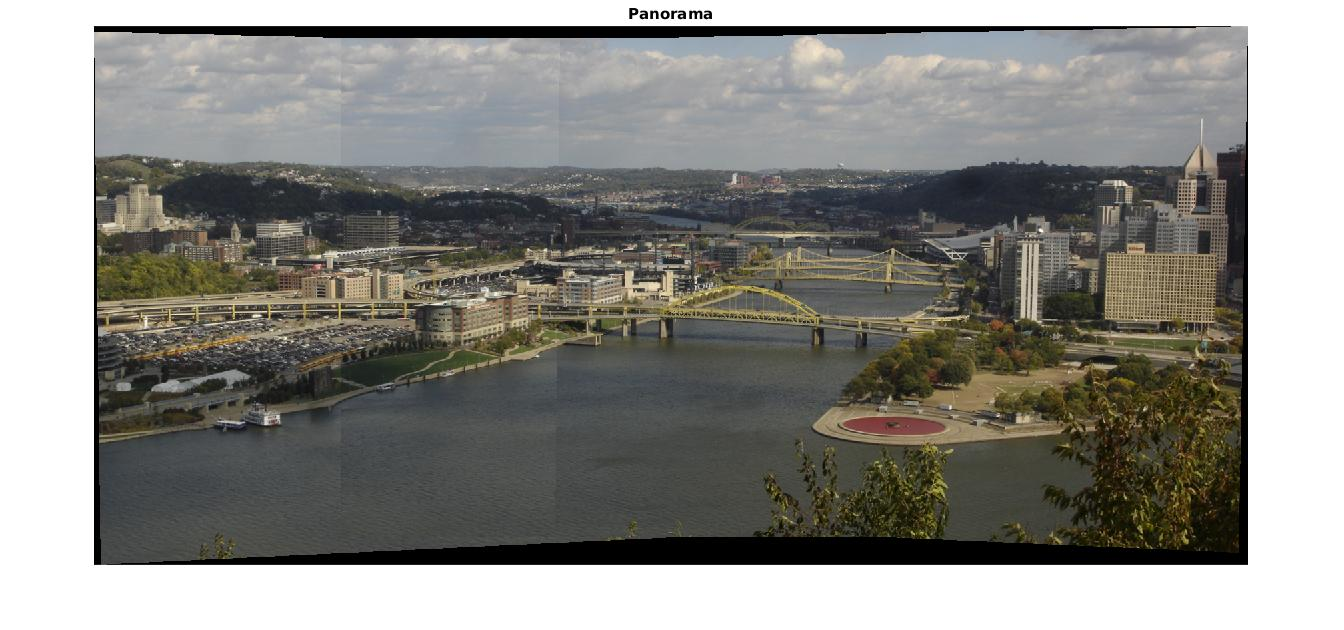
\includegraphics[scale=0.4]{pitt_panorama.jpg}
\label{fig_pittPanorama}
\caption{The final stitched image of the Pittsburgh skyline}
\end{figure}

\begin{figure}[H]
\centering
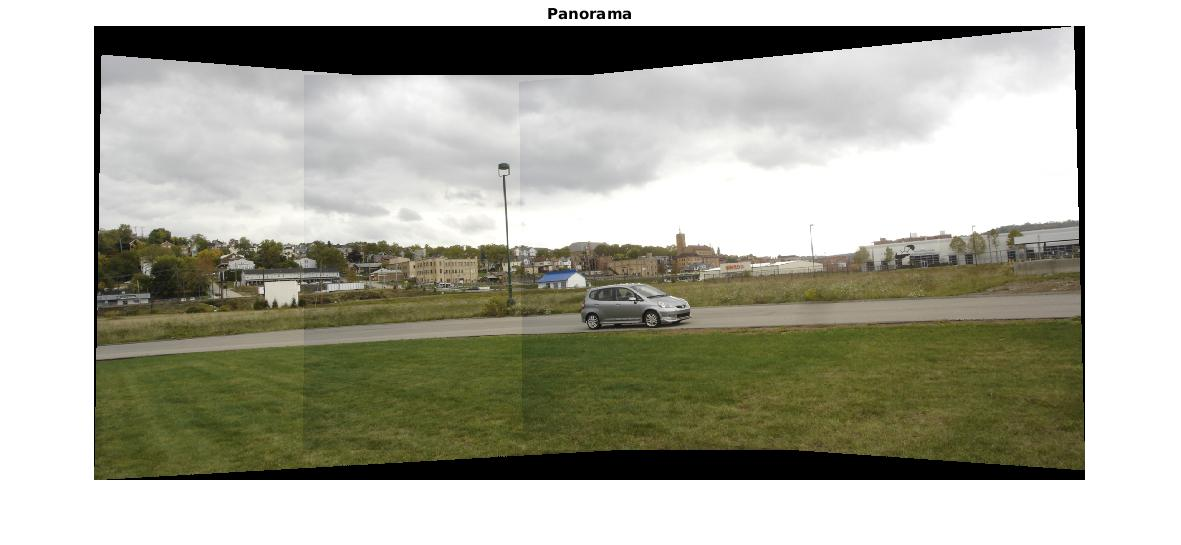
\includegraphics[scale=0.4]{car_panorama.jpg}
\label{fig_carPanorama}
\caption{Another stitching result}
\end{figure}



\end{document}